\documentclass[,man,floatsintext]{apa6}
\usepackage{lmodern}
\usepackage{amssymb,amsmath}
\usepackage{ifxetex,ifluatex}
\usepackage{fixltx2e} % provides \textsubscript
\ifnum 0\ifxetex 1\fi\ifluatex 1\fi=0 % if pdftex
  \usepackage[T1]{fontenc}
  \usepackage[utf8]{inputenc}
\else % if luatex or xelatex
  \ifxetex
    \usepackage{mathspec}
  \else
    \usepackage{fontspec}
  \fi
  \defaultfontfeatures{Ligatures=TeX,Scale=MatchLowercase}
\fi
% use upquote if available, for straight quotes in verbatim environments
\IfFileExists{upquote.sty}{\usepackage{upquote}}{}
% use microtype if available
\IfFileExists{microtype.sty}{%
\usepackage{microtype}
\UseMicrotypeSet[protrusion]{basicmath} % disable protrusion for tt fonts
}{}
\usepackage{hyperref}
\hypersetup{unicode=true,
            pdftitle={Early language experience in a Papuan village},
            pdfauthor={Marisa Casillas, Penelope Brown, \& Stephen C. Levinson},
            pdfkeywords={Child-directed speech, linguistic input, non-WEIRD, vocal maturity, turn
taking, interaction, Papuan},
            pdfborder={0 0 0},
            breaklinks=true}
\urlstyle{same}  % don't use monospace font for urls
\usepackage{graphicx}
% grffile has become a legacy package: https://ctan.org/pkg/grffile
\IfFileExists{grffile.sty}{%
\usepackage{grffile}
}{}
\makeatletter
\def\maxwidth{\ifdim\Gin@nat@width>\linewidth\linewidth\else\Gin@nat@width\fi}
\def\maxheight{\ifdim\Gin@nat@height>\textheight\textheight\else\Gin@nat@height\fi}
\makeatother
% Scale images if necessary, so that they will not overflow the page
% margins by default, and it is still possible to overwrite the defaults
% using explicit options in \includegraphics[width, height, ...]{}
\setkeys{Gin}{width=\maxwidth,height=\maxheight,keepaspectratio}
\IfFileExists{parskip.sty}{%
\usepackage{parskip}
}{% else
\setlength{\parindent}{0pt}
\setlength{\parskip}{6pt plus 2pt minus 1pt}
}
\setlength{\emergencystretch}{3em}  % prevent overfull lines
\providecommand{\tightlist}{%
  \setlength{\itemsep}{0pt}\setlength{\parskip}{0pt}}
\setcounter{secnumdepth}{0}
% Redefines (sub)paragraphs to behave more like sections
\ifx\paragraph\undefined\else
\let\oldparagraph\paragraph
\renewcommand{\paragraph}[1]{\oldparagraph{#1}\mbox{}}
\fi
\ifx\subparagraph\undefined\else
\let\oldsubparagraph\subparagraph
\renewcommand{\subparagraph}[1]{\oldsubparagraph{#1}\mbox{}}
\fi

%%% Use protect on footnotes to avoid problems with footnotes in titles
\let\rmarkdownfootnote\footnote%
\def\footnote{\protect\rmarkdownfootnote}


  \title{Early language experience in a Papuan village}
    \author{Marisa Casillas\textsuperscript{1}, Penelope Brown\textsuperscript{1},
\& Stephen C. Levinson\textsuperscript{1}}
    \date{}
  
\shorttitle{Early language experience in a Papuan village}
\affiliation{
\vspace{0.5cm}
\textsuperscript{1} Max Planck Institute for Psycholinguistics}
\keywords{Child-directed speech, linguistic input, non-WEIRD, vocal maturity, turn taking, interaction, Papuan\newline\indent Word count: XXXXX (XXXX not including references)}
\usepackage{csquotes}
\usepackage{upgreek}
\captionsetup{font=singlespacing,justification=justified}

\usepackage{longtable}
\usepackage{lscape}
\usepackage{multirow}
\usepackage{tabularx}
\usepackage[flushleft]{threeparttable}
\usepackage{threeparttablex}

\newenvironment{lltable}{\begin{landscape}\begin{center}\begin{ThreePartTable}}{\end{ThreePartTable}\end{center}\end{landscape}}

\makeatletter
\newcommand\LastLTentrywidth{1em}
\newlength\longtablewidth
\setlength{\longtablewidth}{1in}
\newcommand{\getlongtablewidth}{\begingroup \ifcsname LT@\roman{LT@tables}\endcsname \global\longtablewidth=0pt \renewcommand{\LT@entry}[2]{\global\advance\longtablewidth by ##2\relax\gdef\LastLTentrywidth{##2}}\@nameuse{LT@\roman{LT@tables}} \fi \endgroup}


\usepackage{lineno}

\linenumbers

\authornote{

Correspondence concerning this article should be addressed to Marisa
Casillas, P.O. Box 310, 6500 AH Nijmegen, The Netherlands. E-mail:
\href{mailto:Marisa.Casillas@mpi.nl}{\nolinkurl{Marisa.Casillas@mpi.nl}}}

\abstract{
To be completed later.


}

\begin{document}
\maketitle

\section{Introduction}\label{intro}

In their first five years of life, children hear an extraordinary amount
of language in a wide variety of interactional contexts. Tracking the
distribution and characteristics of this linguistic input over the day,
across age, and between children is a difficult task. Until recently,
developmental language science has relied on short video recordings of
caregiver-child interaction, at home or in the lab, to get a grasp on
what kinds of language children typically hear. This has been a fruitful
approach in teasing out individual and group-based differences in
interactional style (REFS). However, short recordings are limited in
their insight because they represent only a small slice of the child's
language abilities and experiences (REFS).

Improved recording hardware and advances in speech technology have
recently allowed us to use daylong recordings to get a peek into
children's broader language landscapes. Daylong recordings are made with
a device, usually positioned on the target child's chest, while that
child freely navigates their social environment for most of a waking day
(REFS). This style of audio recording has allowed researchers to track
children's verbal language use across a range of activity and
interlocutor contexts, yielding more representative and generalizable
measures of their language environments (REFS). While daylong recording
collections are typically too large for comprehensive transcription and
annotation, a combination of automated tools, (REFS) sampling techniques
(REFS), and standardized annotation approaches (REFS) can lead to rich,
but efficiently-gained glimpses into the at-home language environment.
However, properly collecting, processing, and archiving daylong data is
not easily achieved and may not be well suited for a range of research
questions (REFS). At time of writing, there are few options for
capturing visual information across the day (but see REFS), limiting
this method primarily to acoustic phenomena (REFS).

Daylong recording methods are still relatively new, and their
reliability and predictive value for language development have not yet
been fully established. For example, one collection of recordings made
in the US Northwest suggests that there is so much variability across
activities and days in basic talk characteristics (e.g., how much speech
comes from what types of speakers) that researchers need several days of
recordings before they can expect their input estimates to stabilize
(Anderson \& Fausey, in prep). Even if one can achieve a reliable
estimate of a language environment measure (e.g., overhearable adult
words per hour), how and why that estimate relates to deeper factors
shaping the learning situation, including caregiving ideologies and
language outcomes, is often indirect at best. Relatedly, meaningful
differences between individual children may be minimized when averaging
across the entirety of the day's high and low moments; it may well be
that a few key interactions throughout the day provide sharper
resolution on individual and group-based differences compared to
whole-day averages.

Recent studies have directly investigated the effect of recording
duration on caregiver speech, finding that short recordings display much
denser, and somewhat different input than longer recordings (Bergelson,
Amatuni, Dailey, Koorathota, \& Tor, 2019; Tamis-LeMonda, Kuchirko, Luo,
Escobar, \& Bornstein, 2017). Bergelson and colleagues (Bergelson et
al., 2019) analyzed the contexts of noun use encountered by 44 6- and
7-month-old children in the US in both hour-long at-home videos and
comparable sub-samples of daylong recordings. They found that, while the
videos tended to have very dense noun-related input and significantly
more nouns embedded in questions, daylong samples contained more nearby
speakers and more noun types (see (Bergelson et al., 2019) for the full
range of differences). Frequently heard nouns were more consistent
across families in the daylong data compared to the video data,
suggesting that daylong data may more more robustly capture stable,
group-level similarities in child-proximal speech. Interestingly,
children heard more dense noun input during their \enquote{peak} hour
for the day compared to the video, which also highlights peak
interactions from daylong recordings as a promising compromise between
ecological validity and concentrated measures of language environment
and development. Importantly, a child's relative rank across a range of
speech environment measures may be stable across recording contexts, at
least for US children (Tamis-LeMonda et al., 2017). Based on these
findings, one could infer that at-home short recordings are influenced
by some (but not all) of the same underlying factors that drive language
patterns during daylong recordings (e.g., caregiver ideologies about
child development, child responsiveness, household composition).

Studies of children growing up in two indigenous Mayan communities of
Southern Mexico (Tseltal and Yucatec Mayan) suggest that short and long
recordings may yield substantial differences in how the speech
environment is characterized (REFS). Previous studies on these
communities have tended to use ethnographic and microanalytic analyses
of short interactions to examine the character of children's speech
environments. They have found that caregivers shape infants' and young
children's worlds such that the children learn to attend to what is
going on around them rather than expecting to be the center of attention
(REFS). Consistent with this goal, direct talk to infants, particularly
from adults, is rare until children themselves begin to elicit responses
from others (REFS). Because young children are often cared for by older
siblings and cousins, a substantial portion of talk to young children
was also expected to come from other children (REFS). Similar
observations have been reported for multiple other distinct (but
ethnolinguistically related) communities in the region (REFS). Following
up on this ethnographic work, Shneidman (REFS) used short videos of
interaction to conduct a quantitative, longitudinal study of the speech
young Yucatec children heard. She found that interactional patterns
aligned well with observations in previous work in that community:
infants were rarely spoken to at first, but their language input
increased enormously with age, mostly due to an influx of speech from
other children (REFS). However, when Casillas and colleagues (REFS) used
daylong recordings with a Tseltal Mayan community, where a similar
caregiver interactional style has been described previously on the basis
of short videos, the pattern of findings diverged from expectations. In
brief, they found that infants and young children were indeed spoken to
rarely, but that there was no increase in speech input with age and the
majority of speech came from adult women, even when children were old
enough to independently follow their older siblings and cousins around
the house. These divergent results betweeh daylong and short video
recordings don't imply that the latter is wrong, only that it is not
representative with respect to the child's language experience over an
entire day.

These findings do raise an important issue faced by developmental
psychology as it continues to expand the study of child language to more
diverse speech communities: when researchers are not members of the
community they are studying, it is difficult to know a priori what is
typical, representative, or meaningful in children's language
experience. By observing as much speech as possible in a context as
ecologically valid as possible and by sampling, annotating, and
analyzing the data on the basis of the most established development
measures we have, researchers using daylong recordings might hope to
approach this issue without first needing to conduct deep ethnographic
studies in the community on caregiving practices and ideologies around
language use and language development (REFS). When studying members of
our own cultural group, we can bridge between simple, observable
behaviors and rich interpretations of, thereby expanding our explanatory
model beyond the measures directly analyzed (e.g., why child-directed
talk might relate to faster vocabulary development). We cannot hope to
gain such enriched understandings cross-culturally without ethnographic
work; and in the absence of such work we must accept that there may be a
dissociation between how we have traditionally understood an
operationalized language behavior (e.g., child-directed speech) and what
drives the use and form of that behavior in a given community or
interactional context (e.g., pedagogical concerns, entertainment of the
caregiver, getting the child to assist). Until there are trained
researchers working on this topic who were born and raised as members of
these communities (what we should be trying to cultivate for the longer
term) this is a quandary we will continue to face.

Pairing ethnographic work with broader-scope studies of children's
language environments may be the most fruitful way to ensure that their
speech environments and speech development are captured well enough to
propose and test meaningful theories cross-culturally. These two methods
have complementary roles to play in exploring the landscape of at-home
language, and neither should be taken to reflect the \enquote{true}
language input for a given child; after all, in the example of Tseltal
above, many interactions with infants during the daylong recordings came
during moments where visitors using a video camera, or even other
community members, would not typically be invited (e.g., after the
parent was roused by the child, who was waking from an afternoon sleep).
If we want to encourage more work on small-scale and/or understudied
language learning contexts, it will be important to continue
establishing how different methods of measuring the input impact the
conclusions that are likely to be made.

In this study we present analyses of daylong recordings from a
small-scale indigenous group, on Rossel Island, Papua New Guinea (PNG),
in which prior ethnographic work has painted a clear picture of early
caregiver-child interaction: child-centric, face-to-face interaction
from the first days of infancy. Based on the prior ethnographic work,
detailed below, we made four predictions about children's speech
environments. First, we predicted that children on Rossel Island would
hear frequent child-directed speech from a wide variety of caregiver
types throughout the day. Second, given how frequently they are passed
between caregivers, we expected to see weaker effects of the subsistence
farming schedule on Rossel children's input than has been found in other
societies (Casillas et al., forthcoming). Third, as children get older,
we expected to see a large increase in the proportion of child-directed
speech coming from other children (see also Shneidman REFS). Fourth, we
expected a large quantity of other-directed speech around them, given
the large number of family numbers typically present. Based on prior
work with daylong recordings with both Western and non-Western
small-scale populations, we additionally expected (a) no age-related
increase in child-directed speech (Scaff, Casillas, Bergelson, REFS),
(b) an age-related decrease in other-directed speech (Casillas,
Bergelson, REFS), and (c) that children's input would be non-uniformly
distributed over the day (Abney, Smith, \& Yu, 2017; Blasi, Schikowski,
Moran, Pfeiler, \& Stoll, in preparation) such that interactional peaks
present a much denser view of their input (Casillas et al.,
forthcoming), similar to that observed in short videos.

In what follows we will review the ethnographic work done with this
community previously, describe our methods for following up on these
findings with daylong recordings, present the current findings, and
discuss the differences that arose. This study was completed as part of
a larger comparative project focusing on children's speech environments
and linguistic development at two sites: the Tseltal Mayan community
mentioned above (Casillas et al., forthcoming) and this Rossel Island
community. Therefore all methods for annotation and analysis in this
study parallel those reported elsewhere for Tseltal Mayan children's
speech environments (Casillas, Brown, \& Levinson, forthcoming).

\section{Method}\label{methods}

\subsection{Corpus}\label{methods-dataset}

The participants in this study live in a collection of small hamlets on
north-eastern Rossel Island, approximately 250 nautical miles off the
southern tip of mainland Papua New Guinea. The traditional language of
Rossel Island is Yélî Dnye, a presumed Papuan isolate, which features a
phonological inventory and set of grammatical features that are unlike
any other in the (predominantly Austronesian) languages of the region.
Rosselers are skilled farmers, cultivating taro, sweet potato, manioc,
yam, coconut, and more for their daily subsistence, with protein coming
from fishing and (occasionally) slaughtering pigs or local animals. Most
children on Rossel Island grow up speaking Yélî Dnye monolingually at
home, beginning to learn English as a second language once they begin
school around age 7 or 8. Children grow up in patrilocal household
clusters (i.e., their family and their father's brothers families),
usually arranged such that there is some shared open space between
households.

During their waking hours, infants are typically carried in a
caregiver's arms as they go about daily activities. Infants, even very
young ones, are frequently passed between different family members (male
and female, young and elderly) throughout the day, returning to the
mother to suckle when hungry. The arc of a typical day for an infant
might include waking, being dressed and fed, then a mix of (a) spending
time with nearby adults or older children as they walk around
socializing and completing tasks with others and (b) more feeding,
perhaps followed by short bouts of sleep in the late morning and
afternoon, usually with the mother. Afternoon meals are cooked from
around 15:00 onward, with another meal time and more socializing at home
before resting for the night. Starting around age two or three, children
also begin to spend a lot of their time in large, independent child
playgroups involving up to 10 or more cousins at a time who freely
travel near and around the village searching for nuts and fruits,
bathing in nearby rivers, and engaging in group games (e.g., tag,
pretend play, etc.).

Interaction with infants and young children on Rossel Island is
initiated by women, men, girls, and boys alike in a face-to-face,
contingency-seeking, and affect-laden style (Brown REFS). Children are
considered a shared responsibility, but also a source of joy and
entertainment for the wider network of caregivers in their community. In
her prior ethnographic work, Brown details some ways in which
interactants make bids for joint attention and act as if the infant can
understand what is being said (REFS). Infants pick up on this pattern of
caregiving, intiating interactions with others twice as frequently as
Tseltal children, who are encouraged instead to be observers of the
interactions going on around them (Brown 2011 REFS). At the same time,
Brown (REFS) documents how Rossel caregivers encourage early
independence in their children, observing their autonomy in choosing
what to do, wear, eat, and say while finding other ways to promote
pro-social behavior (e.g., praise; REFS). Overall, Rossel Island could
be characterized as a child-centered language environment (Ochs \&
Schieffelin 1984; REFS but see Brown \& Casillas REFS), in which
children, even very young ones, are considered interactional and
conversational partners whose interests are allowed to shape the topic
and direction of conversation.

We were interested to investigate the language environment of children
acquiring Yélî Dnye because prior ethnographic work had suggested that
child-directed speech is highly frequent in this community, from mothers
and other adult caregivers, but also from other children. Therefore we
were interested in understanding how children's input environment
influenced their acquisition of this language with all its rare
structures.

The data presented here come from Rossel Island subset of the Casillas
HomeBank Corpus (Casillas, Brown, \& Levinson, 2017), a collection of
raw daylong recordings and more from over 100 children under age four
growing up on Rossel Island and in the Tseltal Mayan community described
elsewhere (Casillas et al. forthcoming). The Rossel Island subcorpus was
collected in 2016 and includes daylong audio recordings and experimental
data from 57 children born to XX mothers. On average, the target
children in these recordings had X--X younger siblings (mean = X; median
= X) and X--X older siblings (mean = X; median = X); most participating
parents were on the younger end of parents in the community (mothers:
mean = XX years; median = XX; range = XX--XX and fathers: mean = XX;
median = XX; range = XX---XX). Based on our demographic data we estimate
that mothers are typically XX years old when they give birth to their
first child (median = XX; range = XX--XX) with an average inter-child
interval of X years (median = X; range = X--X). Notably, however, we
received several reports, including from nursing staff at the local
health clinic, that mothers now are having children younger and closer
together than in generations past. Household size, defined here as the
number of people sharing kitchen and sleeping areas on a daily basis,
ranged between X and XX (mean = X; meadian = X). Households are
clustered into small hamlets which form a wider group of communal
caregivers and playmates. The hamlets themselves are clustered together
into broader patches of patrilocal residents. The average hamlet in our
corpus comprises X households (median = X; range = X--X); assuming an
average of X children under age seven (i.e., not schooling) and X adults
per household, we estimate that there are between XX and XX children and
between XX and XX adults present throughout the day, not including
visitors, visits to neighboring hamlets or other nearby resident areas.
Therefore, while XX\% of the target children in our corpus are first
born to their mothers, they are immediately incorporated into a much
larger pool of young children whose care is divided among numerous
caregivers. Among our participating families, most mothers had finished
primary school (XX\%; X years of education) or secondary school (XX\%; X
years of education), with a few having completed preparatory school
(XX\%; X years of education) or beyond (XX\%; X years of education).
Only XX\% of mothers had less than a primary school education.
Similarly, most fathers had finished primary school (XX\%; X years of
education) or secondary school (XX\%; X years of education), with a few
having completed preparatory school (XX\%; X years of education) or
beyond (XX\%; X years of education), with only XX\% having less than a
primary school education. To our knowledge at the time of recording, all
but two children were typically developing; one showed signs of
significant language delay and one showed signs of multiple
developmental delay (motor, language, intellectual), both children's
delays were consistently observed in follow-up trips in 2018 and 2019.

Dates of birth for children were initially gotten from parent report. We
were able to verify the vast majority of birth dates using the records
at the island health clinic. Because not all mothers give birth at the
clinic and because dates are written by hand, some births are not
recorded, are inaccurately recorded, or otherwise significantly diverge
from what the parents report. In these cases we gathered information
from as many sources as possible and followed up with the families,
often using the dates of neighboring children born around the same time
to home in on the correct date.

The data we present come from 7--9-hour recordings of a waking day at
home for the child. Children wore the recording device, which was an
elastic vest containing a small stereo audio recorder (Olympus WS-832 or
WS-853) and a miniature camera that captured photos of the child's
frontal view at a fixed interval (every 15 seconds; Narrative Clip 1).
The camera was outfitted with a fisheye lens that, while distorting the
images, allowed us to capture 180 degrees of children's frontal view.
This technique allows us to use daylong recordings while also partially
getting around the traditional sacrifice of no visual context, thereby
increasing ease and reliability of our transcrition and annotation.
However, because the camera and recorder are separate devices, we had to
synchronize them manually after the recordings were made. To do this, we
used an external wristwatch to record the current time at start of
recording on each device individually, with accuracy down to the second
(photographed by the camera and spoken into the recorder). The camera
timestamps each photo such that we can calculate the number of seconds
that have elapsed between each one. These timestamps can be used with
the cross-device time synchronization cue to create photo-linked audio
files of each recording, which we then format as video files (see
\url{https://github.com/marisacasillas/Weave} for post-processing
scripts and more information). The informed consent process used with
participants, as well as data collection and storage, were conducted in
accordance with ethical guidelines approved by the Radboud University
Social Sciences Ethics Committee.

\subsection{Data selection and annotation}\label{methods-samples}

From the daylong recordings of XX Rossel children, we selected 10
representative children between ages 0;0 and 3;0 for transcription and
analysis in the current study. The 10 children were selected to be
spread between the target age range (0;0--3;0) while also representing a
range of typical maternal education levels found in the community and
being evenly split between male and female children (see also ACLEW
REFS). For each child we then selected a series of non-overalapping
sub-clips from the day for transription in the following order: nine
randomly-selected 2.5-minute clips, five manually-selected
\enquote{peak} turn-taking activity 1-minute clips, five
manually-selected \enquote{peak} vocal activity 1-minute clips, and one
manually-selected 5-minute expansion of the best one-minute clip, for a
total of 37.5 minutes of transcribed audio for each child (6.25 audio
hours in total). The criteria for manual clip selection are identical to
those described for the parallel study on Tseltal by Casillas and
colleagues (forthcoming).

We were limited to selecting sub-clips from 10 children for analysis
because of the time-intensive nature of transcribing these naturalistic
data; 1 minute of audio typically took us approximately 60--70 minutes
to be segmented into utterances, transcribed, annotated, and loosely
translated into English (\textasciitilde{}400 hours total). Given that
Yélî Dnye is nearly exclusively spoken on Rossel Island, where there is
no electricity and unreliable access to mobile data, transcription could
only be completed over the course of three 4--6 week visits by our
research group to the island in 2016, 2018, and 2019.

We used the ACLEW Annotation Scheme (REFS) in ELAN (ELAN REFS) to
transcribe and annotate all hearable speech---both near and distant---in
the clips. We first segmented out the utterances and ascribed them to
individual speakers (e.g., older brother, mother, aunt, etc.). We then
annotated the vocal maturity of each utterance produced by the target
child (non-canonical babble/canonical babble/single
word/multi-word/unsure) and annotated the addressee of all speech from
other speakers (addressed to the target child/one or more other
children/one or more adults/a mix of adults and children/any
animal/other/unsure). Transcription and annotation was done together by
the first author and one of three community members (all native speakers
of Yélî Dnye). The community-based research assistants personally knew
all the families in the recordings, and were able to use their own
experience, the discourse context, and information from the accompanying
photos in reporting what was said and to whom speech was addressed for
each utterance. Detailed manuals and self-guided training materials,
including a \enquote{gold standard test} for this annotation scheme can
be found at URL (REFS).

In what follows we first analyze the nine randomly selected 2.5-minute
clips from each child to establish a baseline view of their speech
environment, focusing on the effects of child age, time of day,
household size, and number of speakers on the rate of child-directed and
overhearable speech present. Next, we repeat these analyses, focusing
instead only on the turn-taking clips to gain a view of the speech
environment as it appears during the peak interactions for the day. This
latter set of analyses may more closely mirror results from prior
ethnographic work. To demonstrate typical development in this context we
briefly present one measure of language development: a coarse trajectory
mapping children's use of babble, first words, and multi-word
utterances. Finally, we wrap up by integrating the divergent
perspectives on Yélî children's speech environment across methods and
relating these findings to the larger literature on child-directed
speech and its role in language development.

\subsection{Statistical models}\label{statistical-models}

We conducted all analyses in R, using the glmmTMB package to run
generalized linear mixed-effects regressions on our dependent measures
(Brooks et al., 2017; R Core Team, 2018). We used ggplot2 to generate
all plots (Wickham, 2009). The dataset and scripts used to generate this
manuscript and analyses can be found at
\url{https://github.com/marisacasillas/Yeli-CLE}. As explained in
previous work (REFS Casillas et al. forthcoming, Bunce et al, in prep),
child-directed and overhearable speech minutes per hour are naturally
restricted to non-negative (0--infinity) values, causing the
distributional variance of those measures to become non-gaussian
(positively skewed). We therefore use negative binomial regressions,
which can better fit non-negative, overdispersed data (Brooks et al.,
2017; Smithson \& Merkle, 2013). In cases when there were extra zeroes
in the data (e.g., no hearable speech because the child was alone), we
added a zero-inflation model to the regression. This method creates two
models: (a) a binary model to evaluate the likelihood of the variable's
presence (e.g., no vs.~some directed speech) and (b) a count model of
the variable (e.g., \enquote{3} vs. \enquote{5} minutes of directed
speech), with an extra parameter indicating data dispersion. More
conventional, gaussian linear mixed-effects regressions with logged
dependent variables are available in the Supplementary Materials. The
results of those alternative models are qualitatively similar to what we
report here.

\section{Results}\label{results}

\begin{table}[tbp]
\begin{center}
\begin{threeparttable}
\caption{\label{tab:tab1}Demographic overview of the 10 children whose recordings are sampled in the current study, including from left to right: child's age (years;months.days); child's sex (M/F); mother's age (years); level of maternal education (none/primary/secondary/preparatory/university); and the number of people living in the child's household.}
\begin{tabular}{lllll}
\toprule
Age & \multicolumn{1}{c}{Sex} & \multicolumn{1}{c}{Mother's age} & \multicolumn{1}{c}{Level of maternal education} & \multicolumn{1}{c}{People in household}\\
\midrule
00;01.09 & F & 31 & secondary & 8\\
00;03.19 & M & 37 & primary & 9\\
00;04.13 & M & 24 & preparatory & 5\\
00;07.18 & M & 24 & secondary & 5\\
00;09.03 & F & 29 & secondary & 5\\
01;00.29 & F & 30 & primary & 9\\
01;05.02 & M & 25 & secondary & 6\\
01;08.03 & F & 33 & primary & 9\\
02;01.22 & F & 21 & secondary & 4\\
02;11.29 & M & 41 & primary & 8\\
\bottomrule
\end{tabular}
\end{threeparttable}
\end{center}
\end{table}

\begin{figure}
\centering
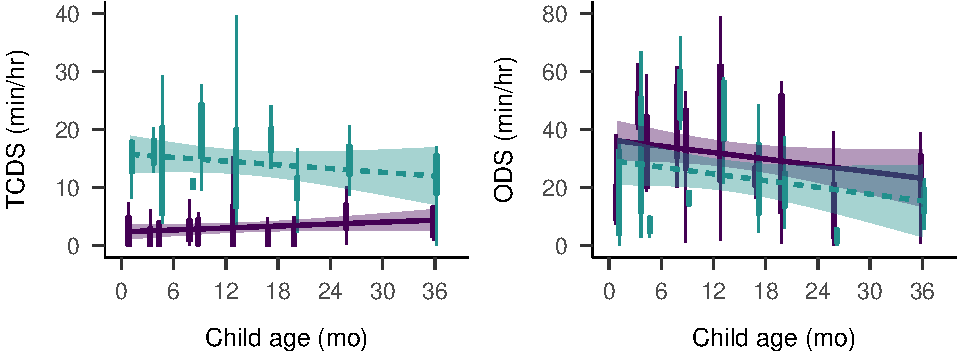
\includegraphics{Yeli-CLE_files/figure-latex/fig2-1.pdf}
\caption{\label{fig:fig2}Recording duration (black line) and sampled clips
(colored boxes) for each of the 10 recordings analyzed, sorted by child
age in months.}
\end{figure}

\begin{verbatim}
## pdf 
##   2
\end{verbatim}

\begin{verbatim}
## pdf 
##   2
\end{verbatim}

\begin{verbatim}
## pdf 
##   2
\end{verbatim}

\begin{verbatim}
## pdf 
##   2
\end{verbatim}

\begin{figure}
\centering
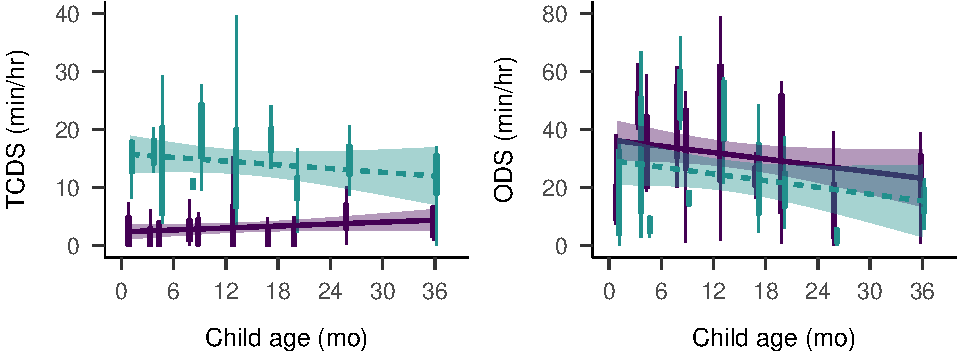
\includegraphics{Yeli-CLE_files/figure-latex/fig3-1.pdf}
\caption{\label{fig:fig3}Estimates of TCDS min/hr (left) and ODS min/hr
(right) across the sampled age range. Each box plot summarizes the data
for one child from the randomly sampled clips (purple; solid) or the
turn taking clips (green; dashed). Bands on the linear trends show 95\%
confidence intervals.}
\end{figure}

\begin{figure}
\centering
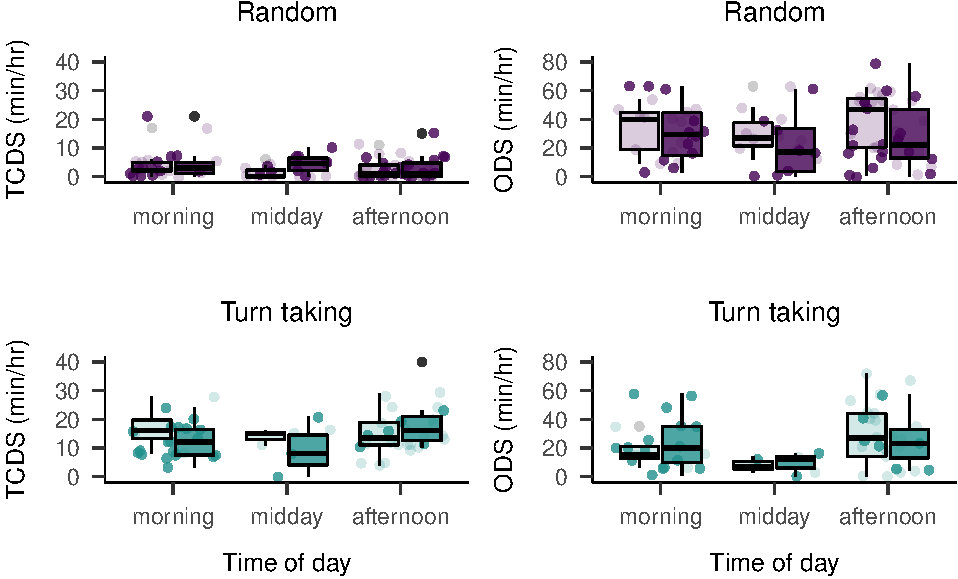
\includegraphics{Yeli-CLE_files/figure-latex/fig5-1.pdf}
\caption{\label{fig:fig5}Estimates of TCDS min/hr (left panels) and ODS
min/hr (right panels) across the recorded day in the random clips (top
panels) and turn-taking (bottom panels) clips. Each box plot summarizes
the data for children age 1;0 and younger (light) or age 1;0 and older
(dark) at the given time of day.}
\end{figure}

\begin{verbatim}
## [1] 3.13
\end{verbatim}

\begin{verbatim}
## [1] 2.95
\end{verbatim}

\begin{verbatim}
## [1] 1.58
\end{verbatim}

\begin{verbatim}
## [1] 6.26
\end{verbatim}

\begin{verbatim}
## [1] 14.45
\end{verbatim}

\begin{verbatim}
## [1] 15.07
\end{verbatim}

\begin{verbatim}
## [1] 9.61
\end{verbatim}

\begin{verbatim}
## [1] 18.73
\end{verbatim}

\begin{verbatim}
## [1] 73.32
\end{verbatim}

\begin{verbatim}
## [1] 78.84
\end{verbatim}

\begin{verbatim}
## [1] 41.41
\end{verbatim}

\begin{verbatim}
## [1] 100
\end{verbatim}

\begin{verbatim}
## [1] 35.9
\end{verbatim}

\begin{verbatim}
## [1] 32.37
\end{verbatim}

\begin{verbatim}
## [1] 20.2
\end{verbatim}

\begin{verbatim}
## [1] 53.78
\end{verbatim}

\begin{verbatim}
## [1] 25.27
\end{verbatim}

\begin{verbatim}
## [1] 19.59
\end{verbatim}

\begin{verbatim}
## [1] 6.68
\end{verbatim}

\begin{verbatim}
## [1] 60.18
\end{verbatim}

\subsection{Vocal maturity}\label{vocal-maturity}

\begin{verbatim}
## pdf 
##   2
\end{verbatim}

\begin{verbatim}
## pdf 
##   2
\end{verbatim}

\begin{verbatim}
## pdf 
##   2
\end{verbatim}

\begin{figure}
\centering
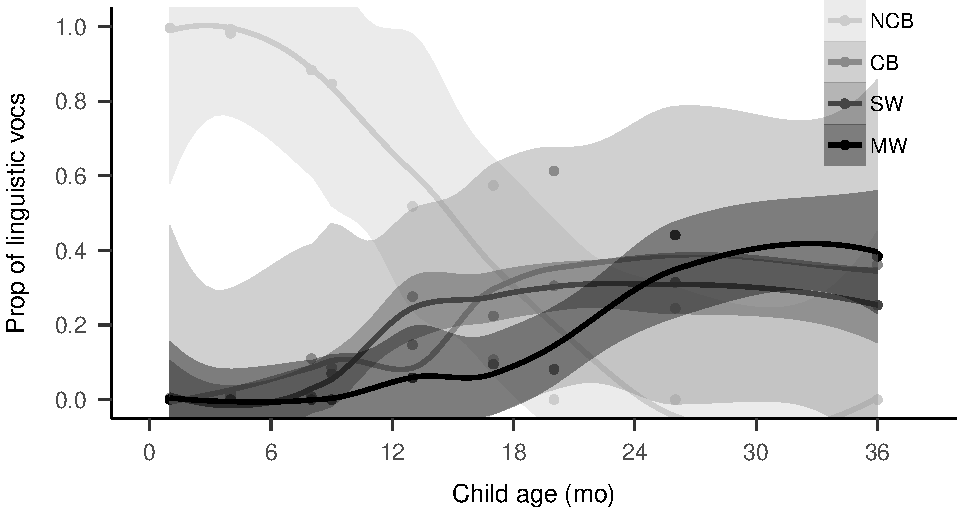
\includegraphics{Yeli-CLE_files/figure-latex/fig6-1.pdf}
\caption{\label{fig:fig6}Proportion of vocalization types used by children
across age (NCB = Non-canonical babble, CB = Canonical babble, SW =
single word utterance, MW = multi-word utterance).}
\end{figure}

\section{Acknowledgements}\label{acknowledgements}

This paper was written using the papaja library in RStudio (Aust \&
Barth, 2018).

\newpage

\section{References}\label{refs}

\begingroup
\setlength{\parindent}{-0.5in} \setlength{\leftskip}{0.5in}

\hypertarget{refs}{}
\hypertarget{ref-abney2017time}{}
Abney, D. H., Smith, L. B., \& Yu, C. (2017). It's time: Quantifying the
relevant time scales for joint attention. In G. Gunzelmann, A. Howes, T.
Tenbrink, \& E. Davelaar (Eds.), \emph{Proceedings of the 39th Annual
Meeting of the Cognitive Science Society} (pp. 1489--1494). London, UK.

\hypertarget{ref-R-papaja}{}
Aust, F., \& Barth, M. (2018). \emph{papaja: Create APA manuscripts with
R Markdown}. Retrieved from \url{https://github.com/crsh/papaja}

\hypertarget{ref-bergelson2019day}{}
Bergelson, E., Amatuni, A., Dailey, S., Koorathota, S., \& Tor, S.
(2019). Day by day, hour by hour: Naturalistic language input to
infants. \emph{Developmental Science}, \emph{22}(1), e12715.
doi:\href{https://doi.org/10.1111/desc.12715}{10.1111/desc.12715}

\hypertarget{ref-blasiIPhuman}{}
Blasi, D., Schikowski, R., Moran, S., Pfeiler, B., \& Stoll, S. (in
preparation). Human communication is structured efficiently for first
language learners: Lexical spikes.

\hypertarget{ref-brooks2017modeling}{}
Brooks, M. E., Kristensen, K., van Benthem, K. J., Magnusson, A., Berg,
C. W., Nielsen, A., \ldots{} Bolker, B. M. (2017). Modeling
zero-inflated count data with glmmTMB. \emph{bioRxiv}.
doi:\href{https://doi.org/10.1101/132753}{10.1101/132753}

\hypertarget{ref-Casillas-HB}{}
Casillas, M., Brown, P., \& Levinson, S. C. (2017). Casillas HomeBank
corpus. doi:\href{https://doi.org/10.21415/T51X12}{10.21415/T51X12}

\hypertarget{ref-R-base}{}
R Core Team. (2018). \emph{R: A language and environment for statistical
computing}. Vienna, Austria: R Foundation for Statistical Computing.
Retrieved from \url{https://www.R-project.org/}

\hypertarget{ref-smithson2013generalized}{}
Smithson, M., \& Merkle, E. (2013). \emph{Generalized linear models for
categorical and continuous limited dependent variables}. New York:
Chapman; Hall/CRC.
doi:\href{https://doi.org/10.1201/b15694}{10.1201/b15694}

\hypertarget{ref-tamislemonda2017power}{}
Tamis-LeMonda, C. S., Kuchirko, Y., Luo, R., Escobar, K., \& Bornstein,
M. H. (2017). Power in methods: Language to infants in structured and
naturalistic contexts. \emph{Developmental Science}, \emph{20}(6),
e12456.
doi:\href{https://doi.org/10.1111/desc.12456}{10.1111/desc.12456}

\hypertarget{ref-R-ggplot2}{}
Wickham, H. (2009). \emph{Ggplot2: Elegant graphics for data analysis}.
Springer-Verlag New York. Retrieved from \url{http://ggplot2.org}

\endgroup


\end{document}
